% Compile from paper/ with: latexmk -pdf main.tex
% Alternatively run pdflatex, bibtex, pdflatex, pdflatex on main.
\documentclass[11pt]{article}
\usepackage[preprint]{acl}
\usepackage{times}
\usepackage[T1]{fontenc}
\usepackage{amsmath,amssymb,booktabs,tikz,balance}
\hypersetup{hidelinks}
\title{When Does It Pay to Exercise an American Put?\\
A Discrete Mathematics Case Study with Berkshire Hathaway}
% Replace the course label with the author's name if desired.
\author{Discrete Mathematics Course Project}
\date{}

\begin{document}
\maketitle

\begin{abstract}
A put option lets its holder sell a share at a fixed price. When the share price falls below that price, exercising pays immediately, yet waiting can still be worth more. We study this choice on a finite graph. A backward pass assigns a value and an action to each state. A forward pass counts only paths on which the option is still alive, yielding the distribution of the first exercise date. A three-step example makes both calculations reproducible by hand. For an illustrative 90-day put on Berkshire Hathaway Class B stock (BRK.B), a 12-step model gives a value of \$13.33 per share and a risk-neutral probability of 46.23\% for exercise before expiration. Enumerating all 4,096 paths recovers the same result. The example shows how a pricing calculation can also explain when, and along which paths, the contract pays.
\end{abstract}

\section{A contract with a choice}
Suppose you own a share worth \$100 and want the right to sell it for \$100 next month. A seller might charge you \$6 today for that right. If the share falls to \$80 at expiration, you can sell for \$100 and gain \$20 relative to selling the share at its market price. After the \$6 purchase price, the option itself has earned \$14, ignoring interest and fees. If the share rises to \$115, you can let the right lapse. The option then costs you the \$6 you paid. These amounts describe the option separately from the gain or loss on the share.

The share is the \emph{underlying}. The agreed sale price is the \emph{strike} $K$, the deadline is the \emph{expiration} or \emph{maturity} $T$, and the purchase price of the right is the \emph{premium}. A \emph{put} gives its buyer the right to sell. A \emph{call} gives its buyer the right to buy. Exercising invokes the right and ends the contract. The seller of an exercised put must buy the shares at the strike. We quote all values per share. For a contract covering 100 shares, a \$6 premium per share costs \$600.

\emph{European} exercise allows a decision at expiration only. \emph{American} exercise also allows a decision earlier in the contract's life \citep{oic}. Consider a put with strike \$100 while the stock trades at \$96. Exercising locks in \$4. Waiting preserves the opportunity to collect more if the stock falls further. It also delays receipt of the money, and the stock could recover. Even though exercise pays something today, the holder needs a way to value the choice that exercise would extinguish.

This paper asks two questions. What is that choice worth today? If the holder follows the optimal exercise rule, at which dates can payment first occur, and with what probability under the pricing model? A time-ordered graph answers both questions. The second answer requires tracking which contracts have survived earlier decisions.

\section{From share prices to a pricing graph}
\subsection{Dates, states, and immediate payoffs}
Let $S_0$ denote today's share price. Divide the remaining $T$ years into $N$ steps of length $\Delta t=T/N$. At each step the current stock price $S$ either rises to $Su$ or falls to $Sd$. In the Cox--Ross--Rubinstein (CRR) model \citep{crr},
\begin{equation}
u=e^{\sigma\sqrt{\Delta t}},\quad d=u^{-1},\quad
R=e^{r\Delta t}.
\label{eq:factors}
\end{equation}
Volatility $\sigma$ measures the annualized dispersion of stock returns. Larger $\sigma$ spreads the two possible prices farther apart. The annual rate $r$ describes an idealized risk-free cash account. One dollar deposited now grows to $R$ dollars one step later. Dividing a future dollar amount by $R$ expresses its value one step earlier.

Index a node by $(i,j)$, where $i$ is the elapsed step count and $j$ counts up moves. Its down and up children are $(i+1,j)$ and $(i+1,j+1)$. The stock price and immediate put payoff there are
\begin{align}
S_{i,j} &= S_0 u^j d^{\,i-j}, \\
H_{i,j} &= \max(K-S_{i,j},0). \label{eq:payoff}
\end{align}
The holder can collect a positive difference when the stock is below the strike (\emph{in the money}). Above the strike, a voluntary sale at $K$ offers no benefit. At expiration, $H$ is therefore the option's entire value. Before expiration, $H$ measures only what immediate exercise can deliver. A premium paid in the past is already spent under either action.

Up then down gives the same stock price as down then up. More generally, all $\binom{i}{j}$ move sequences with $j$ ups end at the same node. Under our constant parameters and stock-price-based payoff they also have the same future choices. This \emph{recombination} makes the graph a directed acyclic graph (DAG) with $i+1$ distinct states in layer $i$. Every edge leads to a later layer.

\subsection{Where the probability comes from}
Consider a claim that pays $V_u$ in the up state and $V_d$ in the down state next step. Buy $\delta$ shares and put $B$ dollars in the cash account, allowing borrowing or short selling. Matching the two payments requires
\[
 \delta Su+BR=V_u,\qquad \delta Sd+BR=V_d.
\]
Subtracting gives $\delta=(V_u-V_d)/(S(u-d))$. The down-state equation then gives $B=(V_d-\delta Sd)/R$. With frictionless trading, a claim and a portfolio with identical future payments must cost the same today. A price difference would let one buy the cheaper position and sell the dearer one while canceling their future obligations. Rearranging the cost $\delta S+B$ gives
\begin{align}
p &= \frac{R-d}{u-d}, \label{eq:p}\\
\delta S+B &= \frac{pV_u+(1-p)V_d}{R}. \label{eq:rep}
\end{align}
The condition $d<R<u$ puts $p$ strictly between zero and one. With this weight the expected growth factor of the stock is $pu+(1-p)d=R$. We write $Q$ for the resulting \emph{risk-neutral} probability law. Its weights reproduce prices in this two-state market. Estimating how often the stock will actually rise is a different statistical question.

\section{Two passes through the graph}
\subsection{Backward induction gives the price}
Write $V_{i,j}$ for the value of a live option at a node, and $C_{i,j}$ for the value of keeping it at least one more step. Initialize the last layer with $V_{N,j}=H_{N,j}$. For $i=N-1,\ldots,0$, apply Equation~\eqref{eq:rep} to the two child values,
\begin{align}
 C_{i,j}&=\frac{(1-p)V_{i+1,j}+pV_{i+1,j+1}}{R},\label{eq:continue}\\
 V_{i,j}&=\max\{H_{i,j},C_{i,j}\}. \label{eq:stop}
\end{align}
The holder exercises when $H_{i,j}>C_{i,j}$ and continues otherwise. This project continues on a tie, including zero versus zero. A tie leaves the price unchanged, but the chosen action can change the recorded time of exercise. At maturity we label a positive payoff as exercise and a zero payoff as worthless expiry.

Backward induction works because each child value already includes the best decision at every subsequent date. Once both child values are available, Equation~\eqref{eq:stop} compares all choices open at their parent. Repeating the argument back to the root gives today's model premium $V_{0,0}$. Exercise is evaluated on grid dates, so a finite tree approximates the exercise opportunities of an American contract.

\subsection{Forward propagation gives the first exercise date}
Let $a_{i,j}$ be the $Q$-probability of reaching $(i,j)$ with the option alive just before the decision. Start with $a_{0,0}=1$ and all other entries zero. A continuing node adds $(1-p)a_{i,j}$ to its down child and $pa_{i,j}$ to its up child. Contributions from different parents add. An exercising node assigns all its incoming probability to a payment at step $i$ and sends nothing onward. Such a node is called \emph{absorbing}.

Let $E_i$ denote the exercise nodes at step $i$, including the positive-payoff nodes when $i=N$. Define $\tau$ as the first exercise step and set $\tau=\infty$ if the option expires worthless. Then
\begin{align}
 Q(\tau=i)&=\sum_{j\,:\,(i,j)\in E_i} a_{i,j}, \label{eq:mass}\\
 V_{0,0}&=\sum_{i=0}^{N}R^{-i}
             \sum_{j\,:\,(i,j)\in E_i}a_{i,j}H_{i,j}. \label{eq:pv}
\end{align}
The first sum reports a fraction of all contracts alive at the root. A conditional probability among contracts still alive at step $i$ would divide it by $\sum_j a_{i,j}$. Equation~\eqref{eq:pv} prices the actual payment at its own date. A path contributes once, at its first exercise, or contributes zero when it expires worthless.

\section{A three-step example by hand}
Take $S_0=K=\$100$, $u=1.25$, $d=0.80$, $R=1.025$, and $N=3$. Here $R$ is specified directly \emph{per step}. Equation~\eqref{eq:p} gives $p=1/2$, making the eight complete paths equally likely. Figure~\ref{fig:tree} shows the stock states. Table~\ref{tab:hand} gives the comparisons at the interior nodes.

\begin{figure}[ht]
\centering
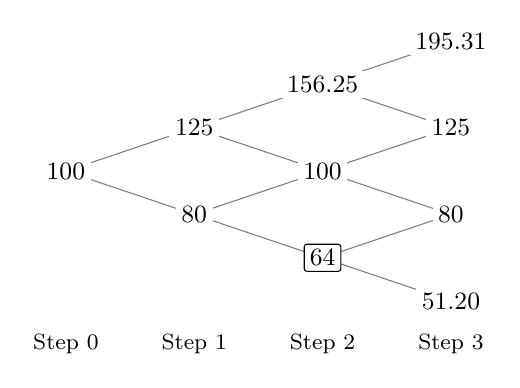
\begin{tikzpicture}[x=1.63cm,y=.55cm,every node/.style={font=\small,inner sep=2pt}]
\foreach \i in {0,1,2} {
  \foreach \j in {0,...,\i} {
    \draw[thin,gray] (\i,{2*\j-\i}) -- ({\i+1},{2*\j-\i-1});
    \draw[thin,gray] (\i,{2*\j-\i}) -- ({\i+1},{2*\j-\i+1});
  }
}
\foreach \i/\y/\s in {0/0/100,1/-1/80,1/1/125,2/0/100,2/2/156.25,3/-3/51.20,3/-1/80,3/1/125,3/3/195.31} {
 \node[fill=white] at (\i,\y) {\s};
}
\node[draw,fill=white,rounded corners=1pt] at (2,-2) {64};
\foreach \i in {0,1,2,3} \node[font=\footnotesize] at (\i,-4) {Step \i};
\end{tikzpicture}
\caption{Stock prices in the hand example. Early exercise at the boxed node removes both outgoing paths from the live option population. The stock can still visit those later prices.}
\label{fig:tree}
\end{figure}

\begin{table}[ht]
\centering\small
\begin{tabular}{rrrrl}
\toprule
Step & Stock & Payoff $H$ & Hold $C$ & Action\\
\midrule
0 & 100.00 & 0 & 13.2093 & Continue\\
1 & 80.00 & 20 & 22.3200 & Continue\\
1 & 125.00 & 0 & 4.7591 & Continue\\
2 & 64.00 & 36 & 33.5610 & Exercise\\
2 & 100.00 & 0 & 9.7561 & Continue\\
2 & 156.25 & 0 & 0.0000 & Continue\\
\bottomrule
\end{tabular}
\caption{Backward decisions before maturity, in dollars per share. Calculations use unrounded values.}
\label{tab:hand}
\end{table}

At step 3 the stock values in ascending order give terminal payoffs of \$48.80, \$20, \$0, and \$0. At the step-2 node with stock \$64, waiting one step is worth $(48.80+20)/(2\times1.025)=\$33.56$. Exercising pays \$36 immediately. At the middle node, the stock is \$100 and waiting is worth $(20+0)/(2\times1.025)=\$9.76$. One step earlier, the stock is \$80 after a down move. Holding is then worth $(36+9.7561)/(2\times1.025)=\$22.32$, exceeding the \$20 available on exercise. The same put can therefore be in the money at two successive dates and call for a different action at each.

For the forward pass let $D$ and $U$ denote a down and an up move. The prefix $DD$ first exercises at step 2 with probability $1/4$. At step 3, the three paths $DDU$, $DUD$, and $UDD$ all end at \$80. The first has already paid \$36 at step 2. Only $DUD$ and $UDD$ still carry a live option and pay \$20, with combined probability $2/8$. The other four live paths expire worthless. Thus the probabilities of early exercise, maturity exercise, and worthless expiry are $1/4$, $1/4$, and $1/2$. Discounting the two possible positive payments independently recovers the root price,
\[
 \frac{(1/4)\,36}{1.025^2}+\frac{(1/4)\,20}{1.025^3}
 = \$13.2093.
\]

\section{A 90-day put on BRK.B}
\subsection{Data and contract specification}
BRK.B denotes Berkshire Hathaway's Class B shares. The archived Nasdaq sample contains 61 closing prices from July~29 through October~22, 2026. The final close supplies $S_0=\$546.97$ \citep{nasdaq}. For consecutive closes $P_{k-1},P_k$, let $x_k=\log(P_k/P_{k-1})$ and let $\bar{x}$ be the mean of the 60 log returns. The annualized historical volatility estimate is
\[
 \hat{\sigma}=\sqrt{252}\,
    \sqrt{\frac{1}{59}\sum_{k=1}^{60}(x_k-\bar{x})^2}
    =0.129078.
\]
The inner square root is the sample standard deviation of daily returns. The factor $\sqrt{252}$ scales daily variability to a trading year under the usual square-root-of-time assumption. This estimate comes from past stock prices. Implied volatility would require an observed option premium and an inverse pricing calculation.

The three-month Treasury par yield on the valuation date was 4.22\% \citep{treasury}. We use $r=0.0422$ directly as a proxy for a constant continuously compounded rate. The contract is illustrative, with $K=\$550$, $T=90/365$ years, $N=12$, and zero dividends. Each exercise interval is 7.5 calendar days. Equations~\eqref{eq:factors} and~\eqref{eq:p} give $u=1.018675$, $d=0.981667$, $R=1.0008675$, and $p=0.518816$.

\subsection{Following one decision through the demo}
At the root, immediate exercise yields $550-546.97=\$3.03$. The next-step down and up states have option values of \$18.4818 and \$8.5795. Their discounted weighted average is \$13.3328 by Equation~\eqref{eq:continue}. Continuing preserves about \$10.30 per share of value above immediate exercise.

Four successive down moves bring the stock to \$507.95. At this node immediate exercise pays \$42.05 and continuation is worth \$41.59. Every preceding node along this path continues. Its entire probability $(1-p)^4=5.3610\%$ therefore becomes the first exercise mass at step 4. One step later, the all-down node has stock \$498.64 and would favor exercise if a contract were alive there. Its only parent already exercised, so its incoming mass is zero. An exercise label on a graph and a positive frequency of exercise at that node are separate outputs.

\begin{table}[ht]
\centering\small
\begin{tabular}{lrr}
\toprule
Step & Alive on arrival (\%) & First exercise (\%)\\
\midrule
0--3 & 100.00 & 0.00\\
4 & 100.00 & 5.36\\
5 & 94.64 & 0.00\\
6 & 94.64 & 5.35\\
7 & 89.29 & 9.72\\
8 & 79.56 & 0.00\\
9 & 79.56 & 5.89\\
10 & 73.67 & 9.26\\
11 & 64.41 & 10.64\\
12 (maturity) & 53.77 & 10.58\\
\bottomrule
\end{tabular}
\caption{BRK.B risk-neutral probabilities relative to the initial population. Each of steps 0 through 3 has the same entries. At step 12 the remaining 43.19\% expire worthless. Totals use unrounded probabilities.}
\label{tab:brkb}
\end{table}

Table~\ref{tab:brkb} shows that 46.23\% exercise early, 10.58\% exercise at maturity, and 43.19\% expire worthless. For example, 10.58\% of the original population exercises at maturity, equivalent to about $10.58/53.77=19.7\%$ of those that reach maturity alive. Summing the discounted payments in Equation~\eqref{eq:pv} gives \$13.3328 per share, matching the backward price.

\subsection{How much is early exercise worth?}
For comparison, give a second put the same inputs and allow exercise only at maturity. Every path then survives to step $N$. The $\binom{N}{j}$ paths ending at node $(N,j)$ each have probability $p^j(1-p)^{N-j}$. Discounting the terminal payments gives the European put value
\[
 V^{\mathrm{E}}_{0,0}=R^{-N}\sum_{j=0}^{N}
 \binom{N}{j}p^j(1-p)^{N-j}H_{N,j}.
\]
For BRK.B this gives \$12.6554 per share. Access to earlier exercise dates adds \$0.6773 to the model premium. The 46.23\% early-exercise probability measures how often this choice is used under $Q$. The \$0.6773 measures how much those opportunities are worth at the valuation date. Many paths can exercise early even when the gain from choosing the better date on each path is modest.

\subsection{Reproduction and scope}
Open \texttt{demo.html} in the project root. In the three-step scenario select step 2 and the \$64 node, then compare the mass at the \$80 maturity node with the three paths that can reach that stock price. In the BRK.B scenario compare the lowest nodes at steps 4 and 5. These two inspections test whether the displayed probabilities follow the first-exercise rule.

From the project root, run \texttt{python -B build\_demo.py} to rebuild the demo and its distribution table from the two bundled data files. At every layer the program checks that incoming mass equals the mass continuing, exercising, or expiring worthless. It checks Equation~\eqref{eq:pv} against the root value, then enumerates all 8 and 4,096 complete paths under the respective computed policies and compares the results at each step. The numerical checks use an absolute tolerance of $10^{-10}$.

The result is exact for the specified finite model. A finer exercise grid, a different volatility window, or different rates can change the stopping distribution. The \$13.33 value is a model premium for the illustrative contract. No option quote or record of holder exercises enters the calculation. A holder seeking to exit in a live market can also sell the option at an executable bid and compare net proceeds after fees \citep{oic}. Inferring actual exercise frequencies would require observations of such decisions and a model of behavior under real-world probabilities.

\section{What discrete mathematics contributes}
Recombination turns a list of price histories into a countable set of states. A tree with $N$ moves has $2^N$ complete paths, yet its recombining graph contains only $(N+1)(N+2)/2$ nodes. In the BRK.B example that is 91 nodes for 4,096 paths. Backward induction visits each node once to choose an action. Forward propagation visits the same nodes in the opposite order to measure the first payment. Each pass takes $O(N^2)$ time, and storing the graph for inspection takes $O(N^2)$ space.

The distinction between the stock and the live contract is what makes the graph informative. At the hand example's \$80 maturity node, counting stock paths gives three possibilities. Enforcing the stopping rule leaves two payable paths. Graph structure explains which histories can be merged, dynamic programming prices the remaining choice, and conservation of probability checks the timing of the payments. Together they connect a present-day premium to an explicit set of future cash flows that a student can trace and verify.

\balance
\bibliography{references}
\end{document}
